
\documentclass[11pt]{article}
\usepackage[margin=0.5in]{geometry}
\usepackage[utf8]{inputenc}
\usepackage{setspace}
\setstretch{1}
\usepackage[english]{babel}
\usepackage[]{amssymb} 
%\usepackage[enable]{darkmode} 
\usepackage{amsmath, amsthm}
\usepackage{mdframed}
\usepackage{pgfplots}
\usepackage{booktabs}
\usepackage{enumitem}
\usepackage{hyperref}
\usetikzlibrary{pgfplots.fillbetween}  
\pgfplotsset{compat=1.17} 
\makeatletter
\newcommand{\tpmod}[1]{{\@displayfalse\pmod{#1}}}
\makeatother

\mdfdefinestyle{problemstyle}{
    innertopmargin=10pt,
    innerbottommargin=10pt,
    innerrightmargin=10pt,
    innerleftmargin=10pt,
    outerlinewidth=1pt,
    topline=true,
    bottomline=true,
    leftline=true,
    rightline=true
}

%custom enviroment for exercises
\newenvironment{exercise}{
    \begin{mdframed}[style=problemstyle]\textcolor{black}{}
}{
    \end{mdframed}
}


\title{TPHYS 121 Workshop Week 5}
\author{}
\date{\vspace{-5ex}}

\begin{document}
\maketitle
\vspace{-10ex}%not a fan of this, but good fix for now

\section*{Module 2 Problems}
\subsection*{Exercise(s) 5.25, 5.26}
\begin{exercise}
    Each of the following describes a situation, draw a free-body diagram
    \begin{enumerate}[label={\alph*}]
        \item Your physics textbook is sliding across the table. 
        \item A steel beam, suspended by a single cable, is being lowered by 
        crane at a steadily decreasing speed.
    \end{enumerate}
\end{exercise}

\subsection*{Exercise 4.16}
\begin{exercise}
    On the Apallo 14 mission to the moon, astronaut Alan Sheperd hit a golf 
    ball with $6$ iron. The free-fall acceleration on the moon is $1/6$ of 
    it's value on earth. Suppose he hit the ball with a speed of $25m/s$ at 
    a $30^{\circ}$ angle above the horizontal.
    \begin{enumerate}[label={\alph*}]
        \item How much farther did the ball travel on the moon than it would 
        have on earth?
        \item For how much more time was the ball in flight?
    \end{enumerate}
\end{exercise}
\subsection*{Exercise 4.19}
\begin{exercise}
    When the moving sidewalk at the airport is broken, as it often seems to 
    be, it takes you to walk $50s$ from your gate to baggage claim. When it is 
    working and you stand on the moving sidewalk the entire way, without 
    walking, it takes $75s$ to travel the same distance. Assuming you weigh
    $100kg$ how long will it take you to travel from the gate to baggage claim 
    if you walk while riding on the moving sidewalk?
\end{exercise}


\section*{Module 3 Problems}
\subsection*{Exercise 7.14}
\begin{exercise}
    The sled dog in the figure sleds A and B across the snow. The coefficient
    of friction between the sleds and snow is $0.10$. If the tension in rope 1
    is $150N$, what is the tension in rope $2$?
\end{exercise}

\begin{figure}[ht!]
    \centering
    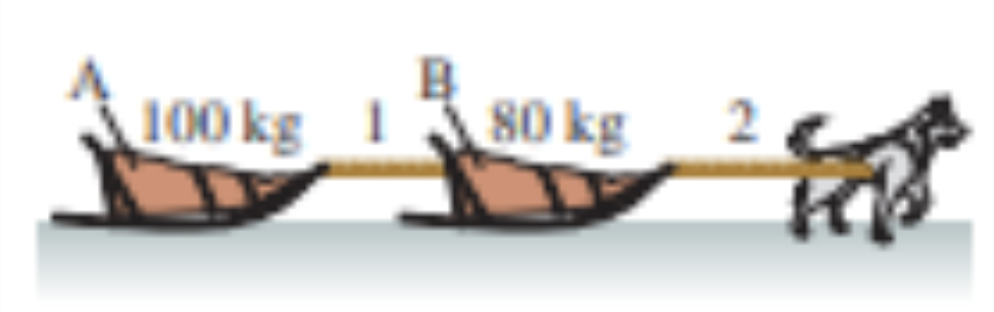
\includegraphics[width=2.5in]{images/exercise714.png}
\end{figure}

\newpage
\subsection*{Exercise 7.15}
\begin{exercise}
    While driving to work last year, I was holding 
    my coffee mug in my left hand while changing the CD 
    with my right hand. Then the cell phone rang, so I 
    placed the mug on the flat part of my dashboard. Then, 
    believe it or not, a deer ran out of the woods and on to 
    the road right in front of me. Fortunately, my reaction time was 
    zero, and I was able to stop from a speed of 
\end{exercise}

\subsection*{Exercise 8.23}
\begin{exercise}
    While at the county fair, you decide to ride the Ferris wheel. 
    Having eaten too many candy apples and elephant ears, you find the 
    motion somewhat unpleasant. To take your mind off your stomach, you 
    wonder about the motion of the ride. You estimate the radius of the 
    big wheel to be $15m$, and you use your watch to find that each loop 
    around takes $25s$.
    \begin{enumerate}[label=\alph*]
        \item What are your speed and the magnitude of your acceleration?
        \item What is the ratio of your weight at the top of the ride to 
            your weight while standing on the ground?
        \item What is the ratio of your weight at the bottom of the ride 
            to your weight while standing on the ground?
    \end{enumerate}
\end{exercise}

\subsection*{Exercise 6.11}
\begin{exercise}
    The figure bellow shows the force acting on a $2.0kg$ object as it moves
    along the x-axis. The object is at rest at the origin at $t=0s$. What 
    is the acceleration and velocity at $t=6s?$.
\end{exercise}
\begin{figure}[ht!]
    \centering
    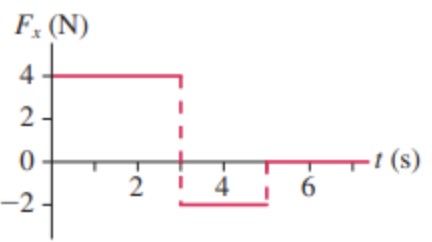
\includegraphics[width=2.5in]{images/figure6_11.png}
\end{figure}


\section*{Additional Resources}
\begin{itemize}
    \item Flipping Physics on youtube: 
        \url{https://www.youtube.com/user/flippingphysics} 
\end{itemize}

\end{document}

